\documentclass[../thesis.tex]{subfiles}

\begin{document}

\section{Convolutional Neural Networks}

Convolutional Neural Networks (CNNs) là một kiến trúc mạng neurons giả định trước rằng dữ liệu đầu vào là dữ liệu ảnh, cho phép trích xuất các thuộc tính trong dữ liệu ảnh đó. Điều này khiến cho việc tính toán trở nên hiệu quả và giảm đáng kể số lượng tham số trong mạng.

Không giống như các mạng neurons thông thường, các lớp của CNNs gồm các neurons có dạng ma trận 3 chiều: chiều rộng, chiều cao, chiều sâu. CNNs sử dụng các filters để tính toán trên các điểm ảnh và trích xuất các đặc trưng có ích cho việc phân lớp.\cite{cs231n}
\begin{figure}[!htb]
	\begin{minipage}{0.48\textwidth}
		\centering
		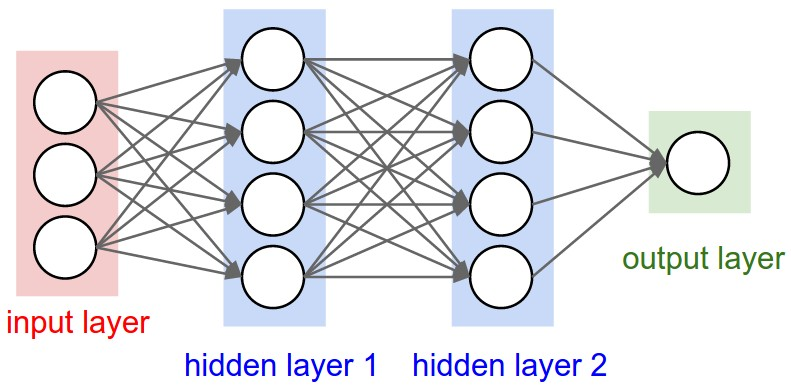
\includegraphics[width=.74\linewidth]{neural_net2.jpeg}
		\caption{Regular Neural Network}\label{Fig:NN}
	\end{minipage}\hfill
	\begin {minipage}{0.48\textwidth}
		\centering
		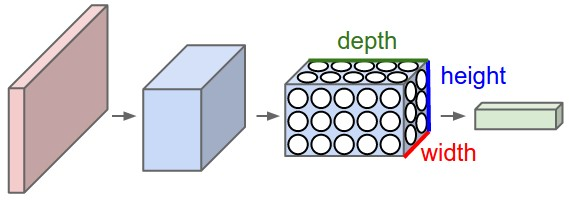
\includegraphics[width=\linewidth]{cnn.jpeg}
		\caption{Convolutional Neural Network}\label{Fig:CNN}
	\end{minipage}
\end{figure}

Các CNNs gồm 3 thành phần chính \cite{tfcnn}: 

\begin{itemize}
  \item Lớp convolutional: sử dụng các convolution filters để tính toán trên ảnh đầu vào, tại mỗi vùng trên ảnh, layer này thực hiện một số phép toán để tạo ra một giá trị duy nhất cho feature map đầu ra. Lớp convolutional thường sử dụng hàm kích hoạt ReLU cho feature map đầu ra.
  \item Lớp pooling: thường nằm sau một convolutional layer để làm giảm kích cỡ (chiều rộng, chiều cao) của feature map để giảm thời gian tính toán. Một thuật toán pooling thường được sử dụng là max pooling.
  \item Dense (fully-connected) layers: thực hiện việc phân lớp dựa trên feature map được trích xuất từ lớp convolutional và lớp pooling.
\end{itemize}

\begin{figure}[!htb]
	\begin{minipage}{0.48\textwidth}
		\centering
		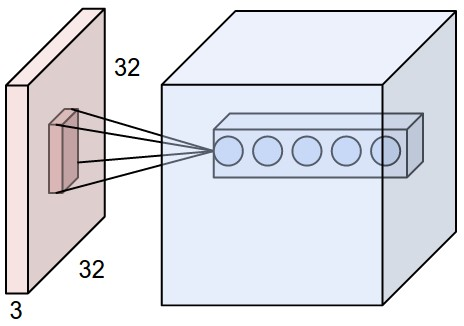
\includegraphics[width=.82\linewidth]{depthcol.jpeg}
		\caption{Regular Neural Network}\label{Fig:depthcol}
	\end{minipage}\hfill
	\begin {minipage}{0.48\textwidth}
		\centering
		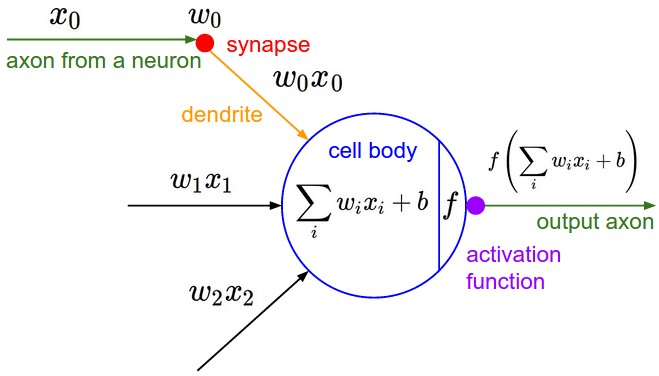
\includegraphics[width=\linewidth]{neuron_model.jpeg}
		\caption{Convolutional Neural Network}\label{Fig:neural_model}
	\end{minipage}
\end{figure}

\section{Region-based Convolutional Neural Networks}

\end{document}